\subsection{HotpotQA Environment}
\label{subsec:hotpotqa}
% \begin{figure}[h]
% \end{figure}
\begin{wrapfigure}{r}{0.45\columnwidth}
\vspace{-10pt}
    \centering
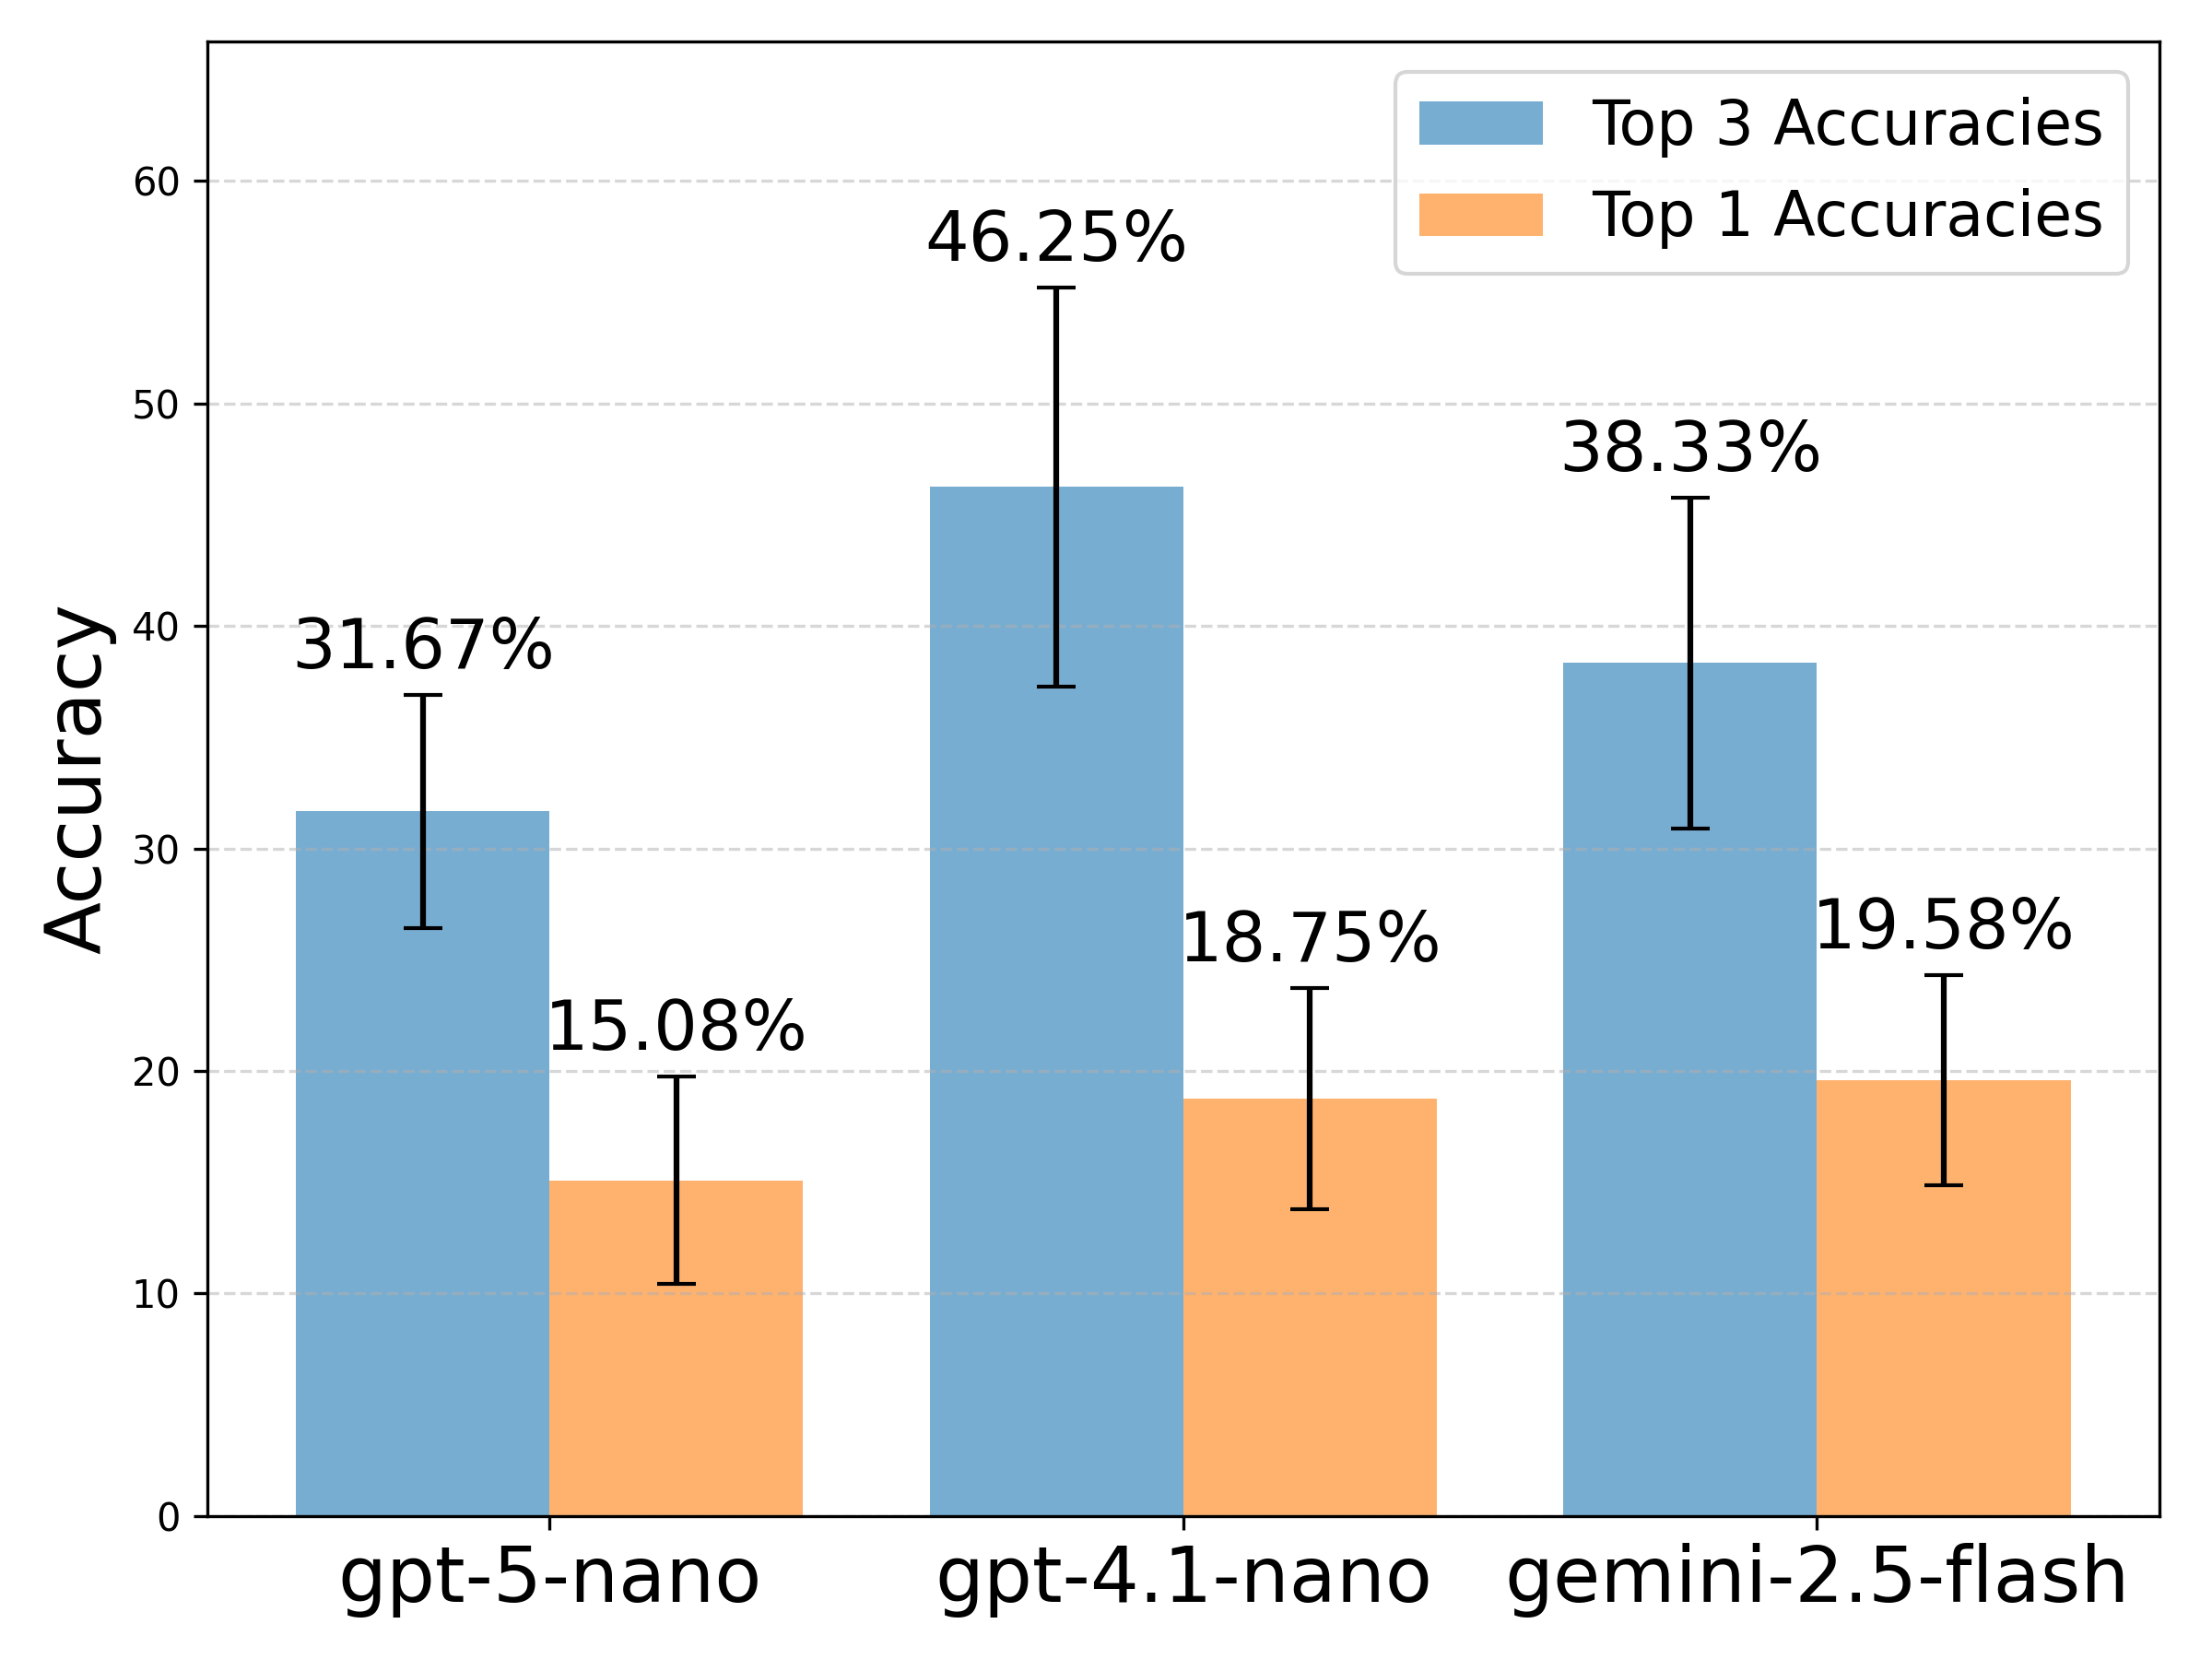
\includegraphics[width=0.9\linewidth]{figures/hotpotqa/accs_gemini-2.5-flashnew.png}
    \caption{Accuracy with gemini-2.5-flash as the Actor. Speculating multiple actions ($k=3$) yields higher accuracy than predicting a single action.}% suggesting that the number of speculative actions can be an effective hyperparameter to tune}
    \label{fig:hotpotqa_accs}
    \vspace{-10pt}
\end{wrapfigure}
We further evaluate our framework on HotpotQA, a setting where the main performance bottleneck arises from information retrieval latency. In this example, the agent must answer multi-hop questions through sequential Wikipedia API calls~\citep{yang2018hotpotqadatasetdiverseexplainable}, mirroring real-world agentic workflows with high round-trip network latency. In this setting, the Speculator predicts likely Wikipedia content while the actual API call executes. Parallelism allows the agent to continue reasoning on provisional information rather than blocking on API latency. % We leave the details of the experimental setup to
See Appendix~\ref{app:hotpotqa} for details about our experimental setup.

We evaluate on the accuracy of the predicted API calls. As shown in Figure \ref{fig:hotpotqa_accs}, the Speculator successfully predicts ground truth API call up to $46\%$ of the time with top-3 prediction. This accuracy improves significantly from top-1 to top-3 predictions, yielding substantial accuracy gains with modest speculation width increase. Our speculation provides value by precomputing reasoning paths during otherwise idle API waiting time. 
